\documentclass[aspectratio=169,11pt]{beamer}

\usepackage[utf8]{inputenc}
\usepackage[T1]{fontenc}
\usepackage{amsmath,amssymb}
\usepackage{appendixnumberbeamer}
\usepackage{xcolor}
\usepackage{tikz}
\usetikzlibrary{arrows.meta,positioning}

% ---------- Tema e colori ----------
\usetheme{default}
\definecolor{navy}{RGB}{18,45,82}
\definecolor{steel}{RGB}{68,105,143}
\definecolor{brick}{RGB}{150,50,40}
\definecolor{lightbg}{RGB}{243,246,250}

\setbeamercolor{structure}{fg=navy}
\setbeamercolor{palette primary}{fg=white,bg=navy}
\setbeamercolor{palette secondary}{fg=white,bg=steel}
\setbeamercolor{palette tertiary}{fg=white,bg=navy}
\setbeamercolor{palette quaternary}{fg=white,bg=navy}
\setbeamercolor{title}{fg=white,bg=navy}
\setbeamercolor{frametitle}{fg=white,bg=navy}
\setbeamercolor{block title}{fg=white,bg=steel}
\setbeamercolor{block body}{fg=black,bg=lightbg}
\setbeamercolor{alerted text}{fg=brick}
\setbeamercolor{background canvas}{bg=white}
\setbeamercolor{footline}{fg=steel}
\setbeamerfont{frametitle}{series=\bfseries}
\setbeamertemplate{navigation symbols}{}
\setbeamertemplate{footline}{%
	\hfill\usebeamercolor[fg]{footline}\small\insertframenumber\,/\,\inserttotalframenumber\hspace{2mm}\vspace{2mm}
}
\setbeamertemplate{itemize item}{\raisebox{0.15em}{\tiny$\blacktriangleright$}}

\title[Strutture Hamiltoniane C*-Algebriche]{Strutture Hamiltoniane nella Ricostruzione\\ C*-Algebrica della Meccanica Classica e Quantistica}
\author{Tommaso Pedroni}
\institute{Dipartimento di Fisica ``A. Volta'' \\ Relatore: Prof. Claudio Dappiaggi}
\date{Anno Accademico 2025--2026}

\begin{document}
	
	% ============ TITOLO (non conta) ============
	\begin{frame}
		\titlepage
	\end{frame}
	
	
	
	% ============ 1. IL PROBLEMA E LA STRATEGIA ============
	\begin{frame}{Il problema e la strategia}
		\begin{itemize}
			\item Meccanica classica: spazio delle fasi, parentesi di Poisson. Meccanica quantistica: spazio di Hilbert, commutatore. Stessa dinamica hamiltoniana, stesso teorema di Noether, in due linguaggi formalmente incompatibili.
			\item Esiste un linguaggio più primitivo, comune a entrambe le teorie?
			\item Strategia Algebrica: non un oggetto geometrico, ma le osservabili fisiche stesse. Si sommano, si moltiplicano, hanno una coniugazione naturale e una norma compatibile risultando in una \textbf{C*-algebra}.
			\item Capitolo 1: Meccanica classica da un'algebra commutativa.
			\item Capitolo 2: Meccanica quantistica da un'algebra non commutativa. 
			\item Capitolo 3: Geometrizzazione dello spazio di Hilbert.
		\end{itemize}
	\end{frame}
	
	% ============ CAPITOLO 1 ============
	
	% ---- 2. Spazio delle fasi ----
	\begin{frame}{Lo spazio delle fasi}
		\begin{itemize}
			\item Lo spazio delle fasi è uno spazio liscio i cui punti sono gli stati del sistema, munita di una forma simplettica $\omega$.
			\item L'energia $H$ genera la dinamica tramite il proprio campo vettoriale hamiltoniano $X_H$, definito da
			\[
			\omega(X_H,\,\cdot\,) = dH.
			\]
			\item Le traiettorie del sistema sono le curve determinate dal campo vettoriale $X_H$.
		\end{itemize}
	\end{frame}
	
	% ---- 3. Parentesi di Poisson ----
	\begin{frame}{Le parentesi di Poisson}
		\begin{itemize}
			\item Valutando $\omega$ sui campi hamiltoniani di due osservabili $f,g$ si ottiene una parentesi antisimmetrica,
			\[
			\{f,g\} = \omega(X_f,X_g), \qquad \dot f = \{f,H\}.
			\]
		\end{itemize}
		\begin{block}{Equazioni di Hamilton tramite Parentesi di Poisson}
			\centering
			\[
			\dot q^i = \{q^i,H\} = \frac{\partial H}{\partial p_i}, \qquad \dot p_i = \{p_i,H\} = -\frac{\partial H}{\partial q^i}
			\]
		\end{block}
		\begin{itemize}
			\item Gli osservabili vengono identificati con le funzioni lisce reali $C^\infty(M;\mathbb{R})$ che sono immerse nella $C^*$-algebra $C^0(M; \mathbb{C})$.
		\end{itemize}
	\end{frame}
	
	% ---- 4. Gelfand-Naimark, con riquadro ----
	\begin{frame}{Il teorema di Gelfand--Naimark}
	\begin{itemize}
		\item Lo spazio degli stati puri relativi alla $C^*$-algebra $\mathfrak{A}$ è chiamato \textit{lo spettro} $X = \sigma(\mathfrak{A})$.
	\end{itemize}
	\begin{block}{Il teorema di Gelfand--Naimark}
		\centering
		\[
		C^*\text{-algebra commutativa } \mathfrak{A} \qquad\Longrightarrow\qquad \mathfrak{A} \;\cong\; C_0\big(X\big)
		\]
	\end{block}
	\begin{itemize}
		\item Partendo dalla sola algebra astratta si ottengono i punti dello spazio delle fasi: gli stati puri del sistema.
	\end{itemize}
\end{frame}
	
	% ---- 5. Il limite della costruzione ----
	\begin{frame}{Un ingrediente esterno}
		\begin{itemize}
			\item Lo spettro così ottenuto è solo uno spazio topologico: nessuna nozione di derivata, quindi nessuna parentesi di Poisson.
			\item Per scriverla serve scegliere una sottoalgebra densa di funzioni lisce, una scelta che l'algebra C* non fissa da sola.
		\end{itemize}
		\vspace{0.4cm}
		\alert{La parentesi di Poisson non è intrinseca all'algebra ma va importata dall'esterno.}
	\end{frame}
	
	% ============ CAPITOLO 2 ============
	
	% ---- 6. Costruzione dell'algebra degli osservabili, a riquadretti ----
	\begin{frame}{La costruzione dell'algebra degli osservabili}
		Punto di vista operativo, alla Bohr: dai due soli dati primitivi dell'esperimento ossia preparazioni e misure, l'algebra si costruisce in successione, senza mai assumere uno spazio di Hilbert.
		
		\vspace{0.25cm}
		\begin{columns}[T,onlytextwidth]
			\column{0.48\textwidth}
			\begin{block}{1. Potenze e Somme}
				\centering\footnotesize
				\vspace{0.15cm}
				$\quad A^n, \quad A^0 \equiv \mathbb{1}, \quad A+B$
				\vspace{0.15cm}
			\end{block}
			\vspace{0.2cm}
			\begin{block}{3. Immersione in $C^*$-algebra}
				\centering\footnotesize
				\vspace{0.1cm}
				$A \circ B = \dfrac12 (AB + BA)$
			\end{block}
			
			\column{0.48\textwidth}
			\begin{block}{2. Prodotto di Jordan}
				\centering\footnotesize
				\vspace{0.1cm}
				$A \circ B := \dfrac{1}{2}\big((A{+}B)^2 {-} A^2 {-} B^2\big)$
			\end{block}
			\vspace{0.2cm}
			\begin{block}{4. Parentesi di Poisson}
				\centering\footnotesize
				\vspace{0.1cm}
				$\{A,B\} := \dfrac{1}{i\hbar}[A,B]$
			\end{block}
		\end{columns}
		
		\vspace{0.3cm}
		Da riscalamento e quadrato delle osservabili emergono, in successione, il prodotto di Jordan, la parentesi di Poisson e infine il prodotto associativo di una C*-algebra: nulla impone che sia commutativo.
	\end{frame}
	
	% ---- 7. GNS: risultato centrale ----
	\begin{frame}{La costruzione GNS}
		Uno stato è un funzionale lineare che restituisce il valore di aspettazione di un'osservabile. $$\omega(A) = \langle A \rangle, \qquad A \in \mathfrak{A}.$$
		\begin{block}{Gelfand--Naimark--Segal}
			Ogni stato $\omega$ su una C*-algebra $\mathfrak{A}$ genera uno spazio di Hilbert $\mathcal H_\omega$, una rappresentazione $\pi_\omega : \mathfrak{A} \to \mathcal{B}(\mathcal{H}_\omega)$ e un vettore $\Psi_\omega \in \mathcal{H}_\omega$ tali che
			\[
			\omega(A) = \big\langle \Psi_\omega,\, \pi_\omega(A)\,\Psi_\omega \big\rangle \qquad \forall A \in \mathfrak{A}.
			\]
		\end{block}
		I postulati di Dirac--von Neumann, stati come vettori e osservabili come operatori, diventano giustificati.
	\end{frame}
	
	% ============ CAPITOLO 3 ============
	
	% ---- 8. Spazio di Hilbert proiettivo ----
	\begin{frame}{Lo spazio di Hilbert proiettivo}
		\begin{itemize}
			\item Gli stati fisici di un sistema quantistico sono raggi di uno spazio di Hilbert: vettori definiti a meno di fase e di norma.
			\item È lo spazio di Hilbert proiettivo $\mathbb P\mathcal H$ l'oggetto su cui vive davvero la fisica, perché due vettori che differiscono per una fase globale rappresentano lo stesso stato.
			\item Questo spazio proiettivo può essere formalizzato come uno spazio liscio come in meccanica classica.
			\item Gli osservabili, prima rappresentati da operatori $A \in \mathcal{B}(\mathcal{H})$, su questo spazio sono mappe $f: \mathbb{P} \mathcal{H} \to \mathbb{R}$ tali che $f = \langle A \rangle$.
		\end{itemize}
	\end{frame}
	
	% ---- 9. Struttura di Kähler + hbar come curvatura ----
	\begin{frame}{La struttura di Kähler}
		\begin{itemize}
			\item $\mathbb P\mathcal H$ porta con sé una metrica riemanniana $g$ e una forma simplettica $\omega$. La parte simplettica genera la dinamica, come nel capitolo 1. La parte metrica ne racchiude il contenuto statistico.
			\item Fissando su $\mathbb P\mathcal H$ una curvatura sezionale olomorfa costante pari a $1/\hbar$, questo stesso flusso hamiltoniano è l'equazione di Schrödinger.
		\end{itemize}
		\vspace{0.2cm}
		\alert{$\hbar$ è l'inverso di una curvatura dello spazio degli stati.}
		\begin{block}{Schr\"odinger $\iff$ Hamilton}
			\centering
			\[
			\omega\big(X_{\langle H\rangle},\,\cdot\,\big) = d\langle H\rangle \qquad\Longleftrightarrow\qquad i\hbar\,\dot\Psi = H\Psi
			\]
		\end{block}
	\end{frame}
	

	
	% ---- 10. Indeterminazione e regola di Born ----
	\begin{frame}{Indeterminazione e regola di Born}
		\begin{itemize}
			\item L'indeterminazione di un'osservabile $f$ si legge da $g$ che genera la dinamica,
			\item La disuguaglianza di Robertson--Schrödinger è Cauchy--Schwarz per $g$.
		\end{itemize}
		\begin{block}{Indeterminazione su un osservabile}
			\centering
			\[
			(\Delta f)^2 = \frac{\hbar}{2}\, g(X_f,X_f) \qquad (\Delta f)(\Delta k) \geq \frac{\hbar}{2} \sqrt{\omega(X_f, X_k)^2 + g(X_f,X_k)^2}
			\]
		\end{block}
	
		\begin{itemize}
			\item Integrando $g$ lungo la geodetica più breve tra due stati puri si ottiene la loro probabilità di transizione, come il coseno al quadrato della distanza geodetica riscalata da $\hbar$: la regola di Born, qui puramente geometrica.
		\end{itemize}
	\end{frame}
	
	% ============ CONCLUSIONE ============
	
	% ---- 12. Sintesi ----
	\begin{frame}{Sintesi e Sviluppi Futuri}
		\begin{center}
			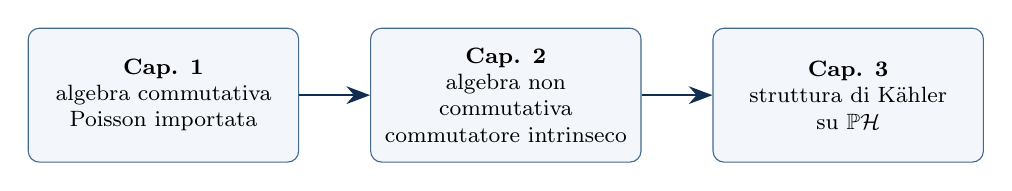
\begin{tikzpicture}[node distance=0.5cm and 0.9cm, every node/.style={font=\footnotesize}]
				\node[draw, rounded corners, fill=lightbg, draw=steel, text width=3.2cm, align=center, minimum height=1.7cm] (c1) {\textbf{Cap. 1}\\ algebra commutativa\\ Poisson importata};
				\node[draw, rounded corners, fill=lightbg, draw=steel, text width=3.2cm, align=center, minimum height=1.7cm, right=of c1] (c2) {\textbf{Cap. 2}\\ algebra non commutativa\\ commutatore intrinseco};
				\node[draw, rounded corners, fill=lightbg, draw=steel, text width=3.2cm, align=center, minimum height=1.7cm, right=of c2] (c3) {\textbf{Cap. 3}\\ struttura di Kähler\\ su $\mathbb P\mathcal H$};
				\draw[-{Stealth[length=3mm]}, thick, navy] (c1) -- (c2);
				\draw[-{Stealth[length=3mm]}, thick, navy] (c2) -- (c3);
			\end{tikzpicture}
		\end{center}
		\vspace{0.5cm}
		La risposta alla domanda iniziale sta nel nucleo algebrico comune alle due teorie. Stessi teoremi, scritti in linguaggi diversi.
		
		\begin{itemize}
			\item Teoria dei campi: infiniti gradi di libertà, rappresentazioni GNS inequivalenti. Qui è trattato solo il caso a dimensione finita.
			\item Estensione a stati misti.
			\item La scelta della sottoalgebra liscia nel capitolo 1 potrebbe risolversi con l'algebra Kähleriana quantistica del capitolo 3.
		\end{itemize}
	\end{frame}

	
	\appendix
	% ============ SLIDE DI BACKUP ============
	\begin{frame}
		\begin{center}
			\Large\textbf{Slide di backup}
		\end{center}
	\end{frame}
	
			% ============ CITAZIONE: APERTURA CAPITOLO 3 ============
	\setbeamercolor{background canvas}{bg=navy}
	\begin{frame}[plain]
		\color{white}
		\vfill
		
		\vspace{0.6cm}
		{\rmfamily\itshape\large ``The correspondence between the quantum and classical theories lies not so much in the limiting agreement when $\hbar \to 0$ as in the fact that the mathematical operations on the two theories obey in many cases the same laws.''}
		
		\vspace{0.7cm}
		\begin{flushright}
			\normalfont\normalsize P.~A.~M.~Dirac (1925)
		\end{flushright}
		\vfill
	\end{frame}
	\setbeamercolor{background canvas}{bg=white}
	
		\begin{frame}
		\frametitle{Il teorema di isomorfismo Lie--Jordan--K\"ahler}
		
		\begin{block}{Le funzioni k\"ahleriane}
			Le funzioni $f=\langle A\rangle$ il cui flusso hamiltoniano preserva l'intera
			struttura di K\"ahler $(\omega,g)$ sono dette \alert{funzioni k\"ahleriane},
			e coincidono esattamente con i valori medi degli operatori autoaggiunti limitati.
		\end{block}
		
		\begin{exampleblock}{Struttura di Lie (forma simplettica $\omega$)}
			\[
			\{\langle A\rangle,\langle B\rangle\} \;=\; \left\langle \frac{1}{i\hbar}[A,B] \right\rangle
			\]
			Parentesi di Poisson tra funzioni k\"ahleriane $\;\cong\;$ commutatore riscalato tra operatori.
		\end{exampleblock}
		
		\begin{exampleblock}{Struttura completa (prodotto di K\"ahler $*_\hbar$)}
			\[
			\langle A\rangle *_\hbar \langle B\rangle \;=\; \langle AB \rangle
			\]
			Il prodotto tra operatori si ricostruisce come prodotto tra funzioni osservabili.
		\end{exampleblock}
		
		\vspace{0.2cm}
		\begin{center}
			\textbf{L'intera algebra degli operatori ha una controparte geometrica esatta.}
		\end{center}
		
	\end{frame}
	
	\begin{frame}{Simmetrie e teorema di Noether}
		\begin{itemize}
			\item Le simmetrie continue, generate da operatori autoaggiunti, producono ancora una mappa momento sullo spazio di Kähler: al generatore di una simmetria corrisponde un'osservabile conservata $J$.
		\end{itemize}
		\begin{block}{}
			\centering
			\[
			\{J,H\} = 0 \qquad\Longleftrightarrow\qquad [J,H]=0
			\]
		\end{block}
		\begin{itemize}
			\item La stessa legge di conservazione, nei due linguaggi del capitolo 1 e del capitolo 2 --- tradotta dalla stessa parentesi.
		\end{itemize}
	\end{frame}
	
\end{document}
	